\documentclass[twoside]{book}

% Packages required by doxygen
\usepackage{fixltx2e}
\usepackage{calc}
\usepackage{doxygen}
\usepackage[export]{adjustbox} % also loads graphicx
\usepackage{graphicx}
\usepackage[utf8]{inputenc}
\usepackage{makeidx}
\usepackage{multicol}
\usepackage{multirow}
\PassOptionsToPackage{warn}{textcomp}
\usepackage{textcomp}
\usepackage[nointegrals]{wasysym}
\usepackage[table]{xcolor}

% Font selection
\usepackage[T1]{fontenc}
\usepackage[scaled=.90]{helvet}
\usepackage{courier}
\usepackage{amssymb}
\usepackage{sectsty}
\renewcommand{\familydefault}{\sfdefault}
\allsectionsfont{%
  \fontseries{bc}\selectfont%
  \color{darkgray}%
}
\renewcommand{\DoxyLabelFont}{%
  \fontseries{bc}\selectfont%
  \color{darkgray}%
}
\newcommand{\+}{\discretionary{\mbox{\scriptsize$\hookleftarrow$}}{}{}}

% Page & text layout
\usepackage{geometry}
\geometry{%
  a4paper,%
  top=2.5cm,%
  bottom=2.5cm,%
  left=2.5cm,%
  right=2.5cm%
}
\tolerance=750
\hfuzz=15pt
\hbadness=750
\setlength{\emergencystretch}{15pt}
\setlength{\parindent}{0cm}
\setlength{\parskip}{3ex plus 2ex minus 2ex}
\makeatletter
\renewcommand{\paragraph}{%
  \@startsection{paragraph}{4}{0ex}{-1.0ex}{1.0ex}{%
    \normalfont\normalsize\bfseries\SS@parafont%
  }%
}
\renewcommand{\subparagraph}{%
  \@startsection{subparagraph}{5}{0ex}{-1.0ex}{1.0ex}{%
    \normalfont\normalsize\bfseries\SS@subparafont%
  }%
}
\makeatother

% Headers & footers
\usepackage{fancyhdr}
\pagestyle{fancyplain}
\fancyhead[LE]{\fancyplain{}{\bfseries\thepage}}
\fancyhead[CE]{\fancyplain{}{}}
\fancyhead[RE]{\fancyplain{}{\bfseries\leftmark}}
\fancyhead[LO]{\fancyplain{}{\bfseries\rightmark}}
\fancyhead[CO]{\fancyplain{}{}}
\fancyhead[RO]{\fancyplain{}{\bfseries\thepage}}
\fancyfoot[LE]{\fancyplain{}{}}
\fancyfoot[CE]{\fancyplain{}{}}
\fancyfoot[RE]{\fancyplain{}{\bfseries\scriptsize Generated by Doxygen }}
\fancyfoot[LO]{\fancyplain{}{\bfseries\scriptsize Generated by Doxygen }}
\fancyfoot[CO]{\fancyplain{}{}}
\fancyfoot[RO]{\fancyplain{}{}}
\renewcommand{\footrulewidth}{0.4pt}
\renewcommand{\chaptermark}[1]{%
  \markboth{#1}{}%
}
\renewcommand{\sectionmark}[1]{%
  \markright{\thesection\ #1}%
}

% Indices & bibliography
\usepackage{natbib}
\usepackage[titles]{tocloft}
\setcounter{tocdepth}{3}
\setcounter{secnumdepth}{5}
\makeindex

% Hyperlinks (required, but should be loaded last)
\usepackage{ifpdf}
\ifpdf
  \usepackage[pdftex,pagebackref=true]{hyperref}
\else
  \usepackage[ps2pdf,pagebackref=true]{hyperref}
\fi
\hypersetup{%
  colorlinks=true,%
  linkcolor=blue,%
  citecolor=blue,%
  unicode%
}

% Custom commands
\newcommand{\clearemptydoublepage}{%
  \newpage{\pagestyle{empty}\cleardoublepage}%
}

\usepackage{caption}
\captionsetup{labelsep=space,justification=centering,font={bf},singlelinecheck=off,skip=4pt,position=top}

%===== C O N T E N T S =====

\begin{document}

% Titlepage & ToC
\hypersetup{pageanchor=false,
             bookmarksnumbered=true,
             pdfencoding=unicode
            }
\pagenumbering{alph}
\begin{titlepage}
\vspace*{7cm}
\begin{center}%
{\Large Documentation \\[1ex]\large 0.\+0.\+1 }\\
\vspace*{1cm}
{\large Generated by Doxygen 1.8.13}\\
\end{center}
\end{titlepage}
\clearemptydoublepage
\pagenumbering{roman}
\tableofcontents
\clearemptydoublepage
\pagenumbering{arabic}
\hypersetup{pageanchor=true}

%--- Begin generated contents ---
\chapter{Class Index}
\section{Class List}
Here are the classes, structs, unions and interfaces with brief descriptions\+:\begin{DoxyCompactList}
\item\contentsline{section}{\hyperlink{classStudent}{Student} \\*\hyperlink{classStudent}{Student} class, four methods et two atts }{\pageref{classStudent}}{}
\end{DoxyCompactList}

\chapter{File Index}
\section{File List}
Here is a list of all files with brief descriptions\+:\begin{DoxyCompactList}
\item\contentsline{section}{\hyperlink{demo_8cpp}{demo.\+cpp} }{\pageref{demo_8cpp}}{}
\item\contentsline{section}{\hyperlink{student_8cpp}{student.\+cpp} }{\pageref{student_8cpp}}{}
\item\contentsline{section}{\hyperlink{student_8h}{student.\+h} }{\pageref{student_8h}}{}
\item\contentsline{section}{\hyperlink{test1_8cpp}{test1.\+cpp} }{\pageref{test1_8cpp}}{}
\item\contentsline{section}{\hyperlink{test2_8cpp}{test2.\+cpp} }{\pageref{test2_8cpp}}{}
\end{DoxyCompactList}

\chapter{Class Documentation}
\hypertarget{classStudent}{}\section{Student Class Reference}
\label{classStudent}\index{Student@{Student}}


\hyperlink{classStudent}{Student} class, four methods et two atts.  




{\ttfamily \#include $<$student.\+h$>$}

\subsection*{Public Member Functions}
\begin{DoxyCompactItemize}
\item 
\hyperlink{classStudent_ababb9f66a55e7ad87a5c5a6be6dda069}{Student} (std\+::string \hyperlink{classStudent_a1d89c28bd42ba9a52da008bb69367171}{name}, bool \hyperlink{classStudent_a110ce4aee2c3c5912933d8e8aa70cc1e}{present}=true)
\begin{DoxyCompactList}\small\item\em Constructor. \end{DoxyCompactList}\item 
std\+::string \hyperlink{classStudent_a1d89c28bd42ba9a52da008bb69367171}{name} () const
\begin{DoxyCompactList}\small\item\em Get students\textquotesingle{} names. \end{DoxyCompactList}\item 
void \hyperlink{classStudent_a9d3a2685df23b5e7cbf59c19c4a1f9b5}{set\+Name} (const std\+::string \&\hyperlink{classStudent_a1d89c28bd42ba9a52da008bb69367171}{name})
\begin{DoxyCompactList}\small\item\em Set student\textquotesingle{}s name. \end{DoxyCompactList}\item 
bool \hyperlink{classStudent_a110ce4aee2c3c5912933d8e8aa70cc1e}{present} () const
\begin{DoxyCompactList}\small\item\em Get the presentation status of a student. \end{DoxyCompactList}\item 
void \hyperlink{classStudent_a4b5a0a2d5e64a49f91f50c790ae3147a}{set\+Present} (bool \hyperlink{classStudent_a110ce4aee2c3c5912933d8e8aa70cc1e}{present})
\begin{DoxyCompactList}\small\item\em Set the presentation status of a student. \end{DoxyCompactList}\item 
std\+::string \hyperlink{classStudent_acd848ed8bb05466e6d96bd387a8326c2}{print} () const
\begin{DoxyCompactList}\small\item\em Print students\textquotesingle{} info. \end{DoxyCompactList}\end{DoxyCompactItemize}
\subsection*{Static Public Member Functions}
\begin{DoxyCompactItemize}
\item 
static int \hyperlink{classStudent_ac8e5bc83d3632e30a849bf0163350d7b}{nb\+\_\+presents} (const std\+::vector$<$ \hyperlink{classStudent}{Student} $>$ \&students)
\begin{DoxyCompactList}\small\item\em Get the number of students who present. \end{DoxyCompactList}\end{DoxyCompactItemize}
\subsection*{Private Attributes}
\begin{DoxyCompactItemize}
\item 
std\+::string \hyperlink{classStudent_adb41893ba19e889e56c559f25fc1a68a}{m\+\_\+name}
\item 
bool \hyperlink{classStudent_a2614877b81d48e893c3ecd519278bbd7}{m\+\_\+present} = true
\begin{DoxyCompactList}\small\item\em student\textquotesingle{}s name \end{DoxyCompactList}\end{DoxyCompactItemize}


\subsection{Detailed Description}
\hyperlink{classStudent}{Student} class, four methods et two atts. 

\subsection{Constructor \& Destructor Documentation}
\mbox{\Hypertarget{classStudent_ababb9f66a55e7ad87a5c5a6be6dda069}\label{classStudent_ababb9f66a55e7ad87a5c5a6be6dda069}} 
\index{Student@{Student}!Student@{Student}}
\index{Student@{Student}!Student@{Student}}
\subsubsection{\texorpdfstring{Student()}{Student()}}
{\footnotesize\ttfamily \hyperlink{classStudent}{Student} (\begin{DoxyParamCaption}\item[{std\+::string}]{name,  }\item[{bool}]{present = {\ttfamily true} }\end{DoxyParamCaption})}



Constructor. 


\begin{DoxyParams}{Parameters}
{\em name} & (string) \\
\hline
{\em present,default} & true (bool) \\
\hline
\end{DoxyParams}


\subsection{Member Function Documentation}
\mbox{\Hypertarget{classStudent_a1d89c28bd42ba9a52da008bb69367171}\label{classStudent_a1d89c28bd42ba9a52da008bb69367171}} 
\index{Student@{Student}!name@{name}}
\index{name@{name}!Student@{Student}}
\subsubsection{\texorpdfstring{name()}{name()}}
{\footnotesize\ttfamily std\+::string name (\begin{DoxyParamCaption}{ }\end{DoxyParamCaption}) const}



Get students\textquotesingle{} names. 

Here is the caller graph for this function\+:
\nopagebreak
\begin{figure}[H]
\begin{center}
\leavevmode
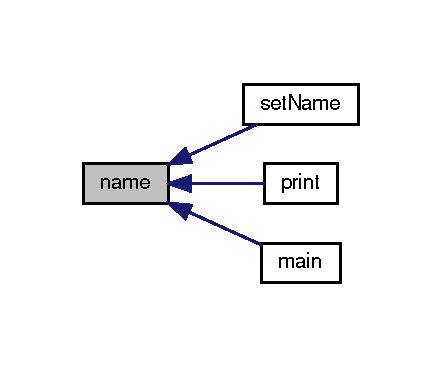
\includegraphics[width=212pt]{classStudent_a1d89c28bd42ba9a52da008bb69367171_icgraph}
\end{center}
\end{figure}
\mbox{\Hypertarget{classStudent_ac8e5bc83d3632e30a849bf0163350d7b}\label{classStudent_ac8e5bc83d3632e30a849bf0163350d7b}} 
\index{Student@{Student}!nb\+\_\+presents@{nb\+\_\+presents}}
\index{nb\+\_\+presents@{nb\+\_\+presents}!Student@{Student}}
\subsubsection{\texorpdfstring{nb\+\_\+presents()}{nb\_presents()}}
{\footnotesize\ttfamily int nb\+\_\+presents (\begin{DoxyParamCaption}\item[{const std\+::vector$<$ \hyperlink{classStudent}{Student} $>$ \&}]{students }\end{DoxyParamCaption})\hspace{0.3cm}{\ttfamily [static]}}



Get the number of students who present. 


\begin{DoxyParams}{Parameters}
{\em students} & (vector) \\
\hline
\end{DoxyParams}
Here is the caller graph for this function\+:
\nopagebreak
\begin{figure}[H]
\begin{center}
\leavevmode
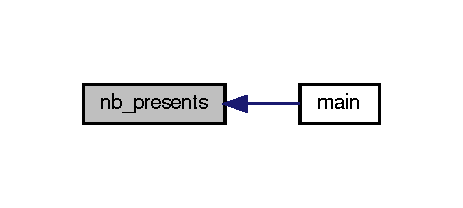
\includegraphics[width=222pt]{classStudent_ac8e5bc83d3632e30a849bf0163350d7b_icgraph}
\end{center}
\end{figure}
\mbox{\Hypertarget{classStudent_a110ce4aee2c3c5912933d8e8aa70cc1e}\label{classStudent_a110ce4aee2c3c5912933d8e8aa70cc1e}} 
\index{Student@{Student}!present@{present}}
\index{present@{present}!Student@{Student}}
\subsubsection{\texorpdfstring{present()}{present()}}
{\footnotesize\ttfamily bool present (\begin{DoxyParamCaption}{ }\end{DoxyParamCaption}) const}



Get the presentation status of a student. 

Here is the caller graph for this function\+:
\nopagebreak
\begin{figure}[H]
\begin{center}
\leavevmode
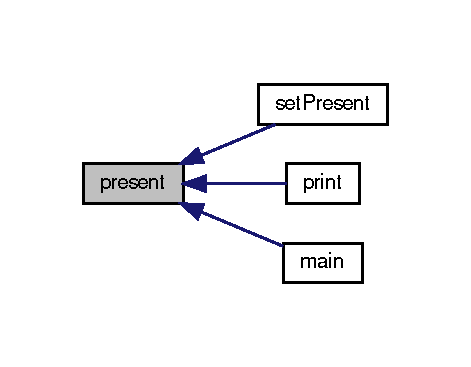
\includegraphics[width=226pt]{classStudent_a110ce4aee2c3c5912933d8e8aa70cc1e_icgraph}
\end{center}
\end{figure}
\mbox{\Hypertarget{classStudent_acd848ed8bb05466e6d96bd387a8326c2}\label{classStudent_acd848ed8bb05466e6d96bd387a8326c2}} 
\index{Student@{Student}!print@{print}}
\index{print@{print}!Student@{Student}}
\subsubsection{\texorpdfstring{print()}{print()}}
{\footnotesize\ttfamily std\+::string print (\begin{DoxyParamCaption}{ }\end{DoxyParamCaption}) const}



Print students\textquotesingle{} info. 

Here is the call graph for this function\+:
\nopagebreak
\begin{figure}[H]
\begin{center}
\leavevmode
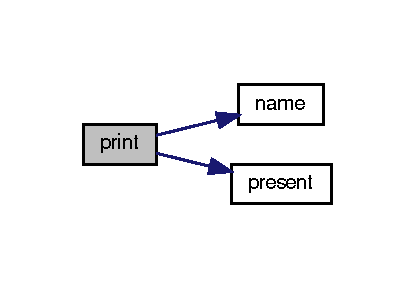
\includegraphics[width=199pt]{classStudent_acd848ed8bb05466e6d96bd387a8326c2_cgraph}
\end{center}
\end{figure}
\mbox{\Hypertarget{classStudent_a9d3a2685df23b5e7cbf59c19c4a1f9b5}\label{classStudent_a9d3a2685df23b5e7cbf59c19c4a1f9b5}} 
\index{Student@{Student}!set\+Name@{set\+Name}}
\index{set\+Name@{set\+Name}!Student@{Student}}
\subsubsection{\texorpdfstring{set\+Name()}{setName()}}
{\footnotesize\ttfamily void set\+Name (\begin{DoxyParamCaption}\item[{const std\+::string \&}]{name }\end{DoxyParamCaption})}



Set student\textquotesingle{}s name. 


\begin{DoxyParams}{Parameters}
{\em name} & (string) \\
\hline
\end{DoxyParams}
Here is the call graph for this function\+:
\nopagebreak
\begin{figure}[H]
\begin{center}
\leavevmode
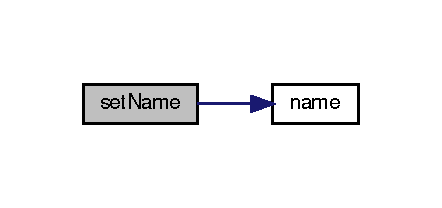
\includegraphics[width=212pt]{classStudent_a9d3a2685df23b5e7cbf59c19c4a1f9b5_cgraph}
\end{center}
\end{figure}
\mbox{\Hypertarget{classStudent_a4b5a0a2d5e64a49f91f50c790ae3147a}\label{classStudent_a4b5a0a2d5e64a49f91f50c790ae3147a}} 
\index{Student@{Student}!set\+Present@{set\+Present}}
\index{set\+Present@{set\+Present}!Student@{Student}}
\subsubsection{\texorpdfstring{set\+Present()}{setPresent()}}
{\footnotesize\ttfamily void set\+Present (\begin{DoxyParamCaption}\item[{bool}]{present }\end{DoxyParamCaption})}



Set the presentation status of a student. 


\begin{DoxyParams}{Parameters}
{\em present} & (bool) \\
\hline
\end{DoxyParams}
Here is the call graph for this function\+:
\nopagebreak
\begin{figure}[H]
\begin{center}
\leavevmode
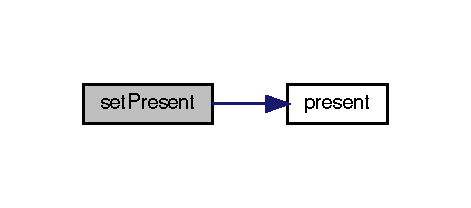
\includegraphics[width=226pt]{classStudent_a4b5a0a2d5e64a49f91f50c790ae3147a_cgraph}
\end{center}
\end{figure}


\subsection{Member Data Documentation}
\mbox{\Hypertarget{classStudent_adb41893ba19e889e56c559f25fc1a68a}\label{classStudent_adb41893ba19e889e56c559f25fc1a68a}} 
\index{Student@{Student}!m\+\_\+name@{m\+\_\+name}}
\index{m\+\_\+name@{m\+\_\+name}!Student@{Student}}
\subsubsection{\texorpdfstring{m\+\_\+name}{m\_name}}
{\footnotesize\ttfamily std\+::string m\+\_\+name\hspace{0.3cm}{\ttfamily [private]}}

\mbox{\Hypertarget{classStudent_a2614877b81d48e893c3ecd519278bbd7}\label{classStudent_a2614877b81d48e893c3ecd519278bbd7}} 
\index{Student@{Student}!m\+\_\+present@{m\+\_\+present}}
\index{m\+\_\+present@{m\+\_\+present}!Student@{Student}}
\subsubsection{\texorpdfstring{m\+\_\+present}{m\_present}}
{\footnotesize\ttfamily bool m\+\_\+present = true\hspace{0.3cm}{\ttfamily [private]}}



student\textquotesingle{}s name 



The documentation for this class was generated from the following files\+:\begin{DoxyCompactItemize}
\item 
\hyperlink{student_8h}{student.\+h}\item 
\hyperlink{student_8cpp}{student.\+cpp}\end{DoxyCompactItemize}

\chapter{File Documentation}
\hypertarget{demo_8cpp}{}\section{demo.\+cpp File Reference}
\label{demo_8cpp}\index{demo.\+cpp@{demo.\+cpp}}
{\ttfamily \#include $<$iostream$>$}\newline
{\ttfamily \#include \char`\"{}student.\+h\char`\"{}}\newline
{\ttfamily \#include $<$vector$>$}\newline
Include dependency graph for demo.\+cpp\+:
\nopagebreak
\begin{figure}[H]
\begin{center}
\leavevmode
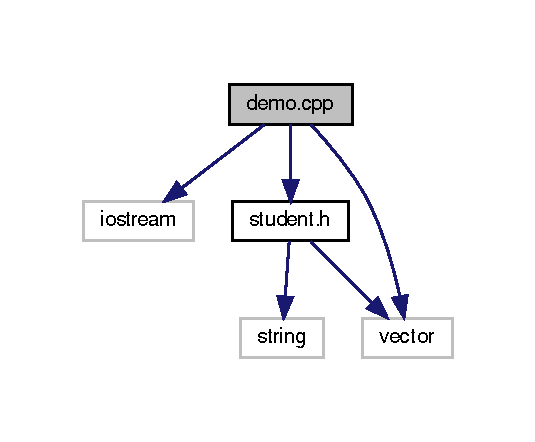
\includegraphics[width=257pt]{demo_8cpp__incl}
\end{center}
\end{figure}
\subsection*{Functions}
\begin{DoxyCompactItemize}
\item 
int \hyperlink{demo_8cpp_a0ddf1224851353fc92bfbff6f499fa97}{main} (int argc, char $\ast$argv\mbox{[}$\,$\mbox{]})
\end{DoxyCompactItemize}


\subsection{Function Documentation}
\mbox{\Hypertarget{demo_8cpp_a0ddf1224851353fc92bfbff6f499fa97}\label{demo_8cpp_a0ddf1224851353fc92bfbff6f499fa97}} 
\index{demo.\+cpp@{demo.\+cpp}!main@{main}}
\index{main@{main}!demo.\+cpp@{demo.\+cpp}}
\subsubsection{\texorpdfstring{main()}{main()}}
{\footnotesize\ttfamily int main (\begin{DoxyParamCaption}\item[{int}]{argc,  }\item[{char $\ast$}]{argv\mbox{[}$\,$\mbox{]} }\end{DoxyParamCaption})}


\hypertarget{student_8cpp}{}\section{student.\+cpp File Reference}
\label{student_8cpp}\index{student.\+cpp@{student.\+cpp}}
{\ttfamily \#include \char`\"{}student.\+h\char`\"{}}\newline
Include dependency graph for student.\+cpp\+:
\nopagebreak
\begin{figure}[H]
\begin{center}
\leavevmode
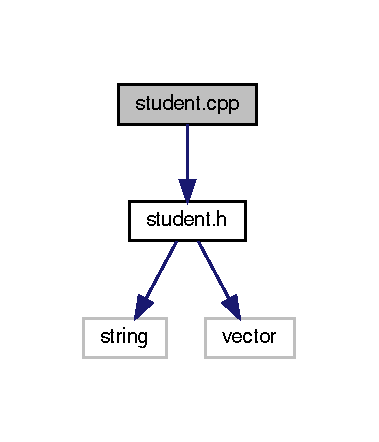
\includegraphics[width=182pt]{student_8cpp__incl}
\end{center}
\end{figure}

\hypertarget{student_8h}{}\section{student.\+h File Reference}
\label{student_8h}\index{student.\+h@{student.\+h}}
{\ttfamily \#include $<$string$>$}\newline
{\ttfamily \#include $<$vector$>$}\newline
Include dependency graph for student.\+h\+:
\nopagebreak
\begin{figure}[H]
\begin{center}
\leavevmode
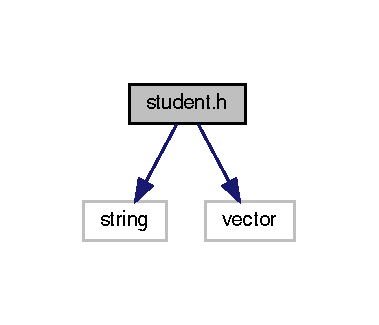
\includegraphics[width=182pt]{student_8h__incl}
\end{center}
\end{figure}
This graph shows which files directly or indirectly include this file\+:
\nopagebreak
\begin{figure}[H]
\begin{center}
\leavevmode
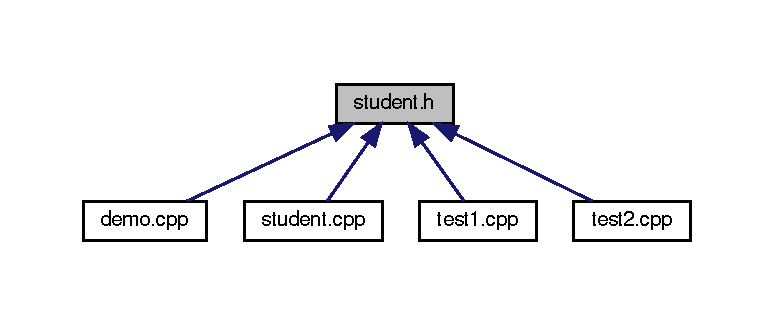
\includegraphics[width=350pt]{student_8h__dep__incl}
\end{center}
\end{figure}
\subsection*{Classes}
\begin{DoxyCompactItemize}
\item 
class \hyperlink{classStudent}{Student}
\begin{DoxyCompactList}\small\item\em \hyperlink{classStudent}{Student} class, four methods et two atts. \end{DoxyCompactList}\end{DoxyCompactItemize}

\hypertarget{test1_8cpp}{}\section{test1.\+cpp File Reference}
\label{test1_8cpp}\index{test1.\+cpp@{test1.\+cpp}}
{\ttfamily \#include $<$iostream$>$}\newline
{\ttfamily \#include \char`\"{}student.\+h\char`\"{}}\newline
Include dependency graph for test1.\+cpp\+:
\nopagebreak
\begin{figure}[H]
\begin{center}
\leavevmode
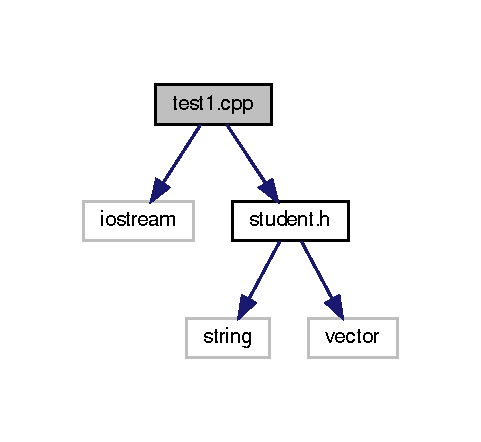
\includegraphics[width=231pt]{test1_8cpp__incl}
\end{center}
\end{figure}
\subsection*{Functions}
\begin{DoxyCompactItemize}
\item 
int \hyperlink{test1_8cpp_a0ddf1224851353fc92bfbff6f499fa97}{main} (int argc, char $\ast$argv\mbox{[}$\,$\mbox{]})
\end{DoxyCompactItemize}


\subsection{Function Documentation}
\mbox{\Hypertarget{test1_8cpp_a0ddf1224851353fc92bfbff6f499fa97}\label{test1_8cpp_a0ddf1224851353fc92bfbff6f499fa97}} 
\index{test1.\+cpp@{test1.\+cpp}!main@{main}}
\index{main@{main}!test1.\+cpp@{test1.\+cpp}}
\subsubsection{\texorpdfstring{main()}{main()}}
{\footnotesize\ttfamily int main (\begin{DoxyParamCaption}\item[{int}]{argc,  }\item[{char $\ast$}]{argv\mbox{[}$\,$\mbox{]} }\end{DoxyParamCaption})}

Here is the call graph for this function\+:
\nopagebreak
\begin{figure}[H]
\begin{center}
\leavevmode
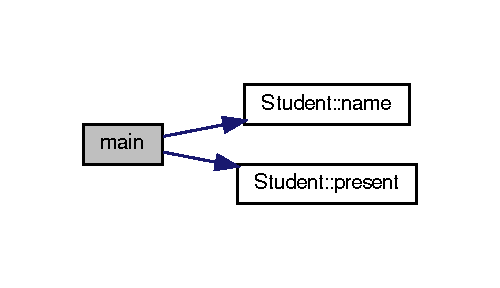
\includegraphics[width=240pt]{test1_8cpp_a0ddf1224851353fc92bfbff6f499fa97_cgraph}
\end{center}
\end{figure}

\hypertarget{test2_8cpp}{}\section{test2.\+cpp File Reference}
\label{test2_8cpp}\index{test2.\+cpp@{test2.\+cpp}}
{\ttfamily \#include $<$iostream$>$}\newline
{\ttfamily \#include \char`\"{}student.\+h\char`\"{}}\newline
{\ttfamily \#include $<$vector$>$}\newline
Include dependency graph for test2.\+cpp\+:
\nopagebreak
\begin{figure}[H]
\begin{center}
\leavevmode
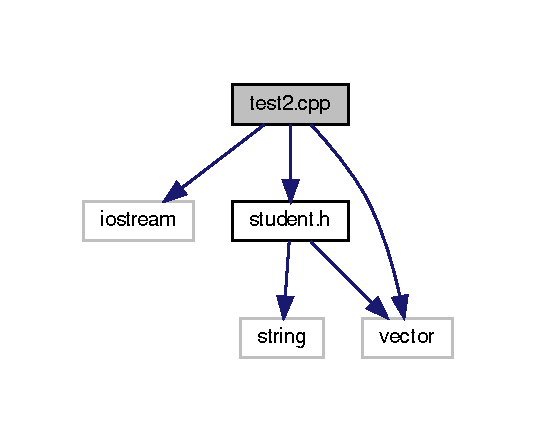
\includegraphics[width=257pt]{test2_8cpp__incl}
\end{center}
\end{figure}
\subsection*{Functions}
\begin{DoxyCompactItemize}
\item 
int \hyperlink{test2_8cpp_a0ddf1224851353fc92bfbff6f499fa97}{main} (int argc, char $\ast$argv\mbox{[}$\,$\mbox{]})
\end{DoxyCompactItemize}


\subsection{Function Documentation}
\mbox{\Hypertarget{test2_8cpp_a0ddf1224851353fc92bfbff6f499fa97}\label{test2_8cpp_a0ddf1224851353fc92bfbff6f499fa97}} 
\index{test2.\+cpp@{test2.\+cpp}!main@{main}}
\index{main@{main}!test2.\+cpp@{test2.\+cpp}}
\subsubsection{\texorpdfstring{main()}{main()}}
{\footnotesize\ttfamily int main (\begin{DoxyParamCaption}\item[{int}]{argc,  }\item[{char $\ast$}]{argv\mbox{[}$\,$\mbox{]} }\end{DoxyParamCaption})}

Here is the call graph for this function\+:
\nopagebreak
\begin{figure}[H]
\begin{center}
\leavevmode
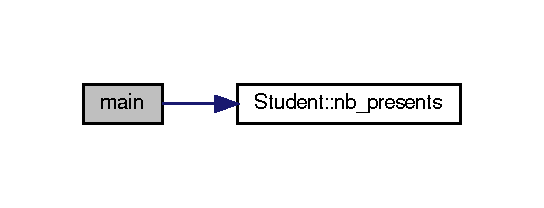
\includegraphics[width=261pt]{test2_8cpp_a0ddf1224851353fc92bfbff6f499fa97_cgraph}
\end{center}
\end{figure}

%--- End generated contents ---

% Index
\backmatter
\newpage
\phantomsection
\clearemptydoublepage
\addcontentsline{toc}{chapter}{Index}
\printindex

\end{document}
